%
% auth: Mattijs Korpershoek
% mail: <mattijs.korpershoek@gmail.com>
%
\section{Methodology}

\currentSectionToc

\subsection{Environment}
\begin{frame}
    \frametitle{Technical environment}
    \begin{minipage}{0.49\textwidth}
    \begin{itemize}
        \item Vim, Tmux, Ssh
        \item C++, Python, Bash, XML
        \item Git, Gerrit, GitHub
        \item Bugzilla
        \item Rational Team Concert
    \end{itemize}
    \end{minipage}
    \begin{minipage}{0.49\textwidth}
        \flushright
        
\includegraphics[height=1.5cm]{./img/vimLogo.png} \hspace{0.2cm}
        
\includegraphics[height=1.5cm]{./img/pythonLogo.png} \\[0.3cm]
        
\includegraphics[height=1.5cm]{./img/githubLogo.png} \hspace{0.2cm}
        
\includegraphics[height=1.5cm]{./img/git-icon.pdf} \\[0.3cm]
        
\includegraphics[height=1.5cm]{./img/bzLogo.png} \hspace{0.2cm}
        
\includegraphics[height=1.5cm]{./img/rtcLogo.jpg}
    \end{minipage}
\end{frame}

\subsection{Agile software development}
\begin{FrameWithSubSection}
    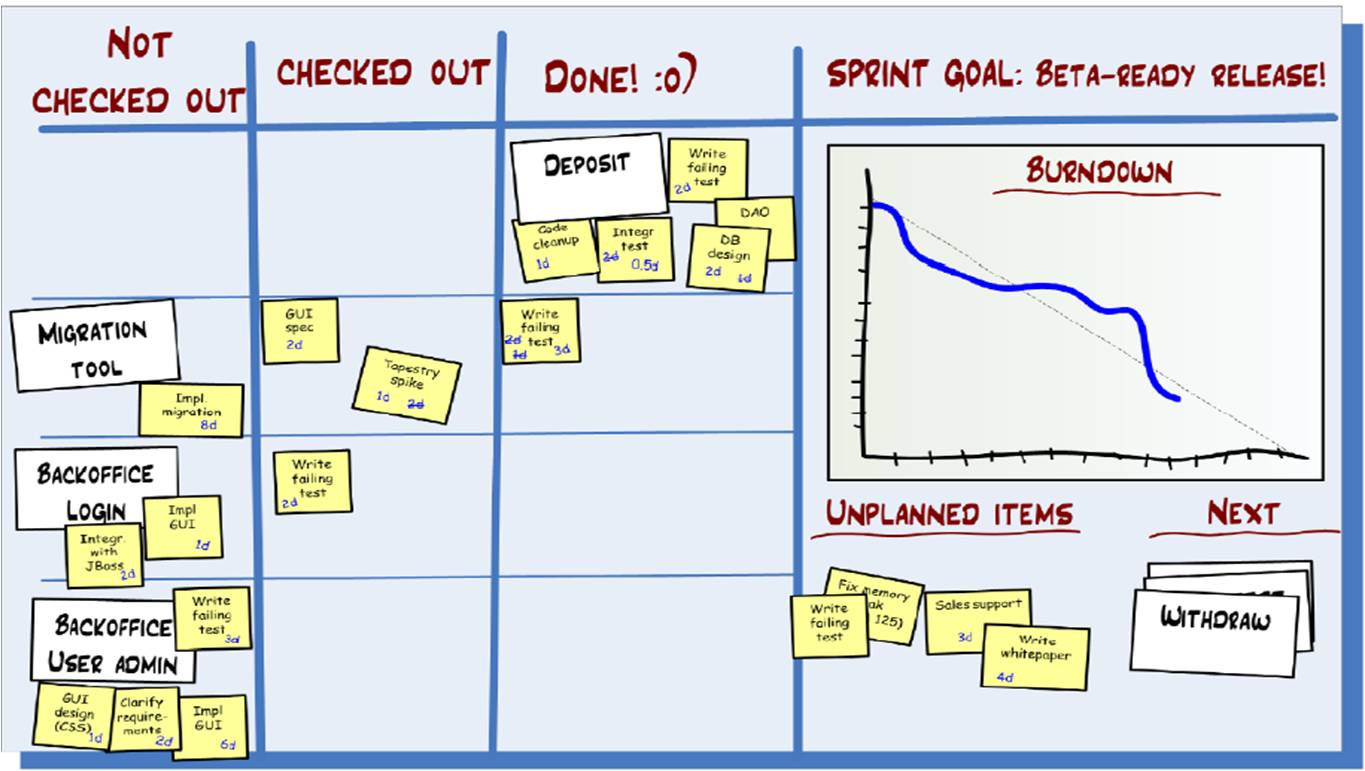
\includegraphics[width=\textwidth]{../../report/src/img/taskboard.jpg}
\end{FrameWithSubSection}

\begin{FrameWithSubSection}
    \frametitle{Agile contributions}
    \begin{minipage}{0.49\textwidth}
        \begin{itemize}
            \item Time management (\emph{Pomodoro technique}, \emph{croissant points})
            \item Pair programming
            \item Human focused retrospectives (\emph{Mad sad glad})
        \end{itemize}
    \end{minipage}
    \begin{minipage}{0.40\textwidth}
        \flushright
        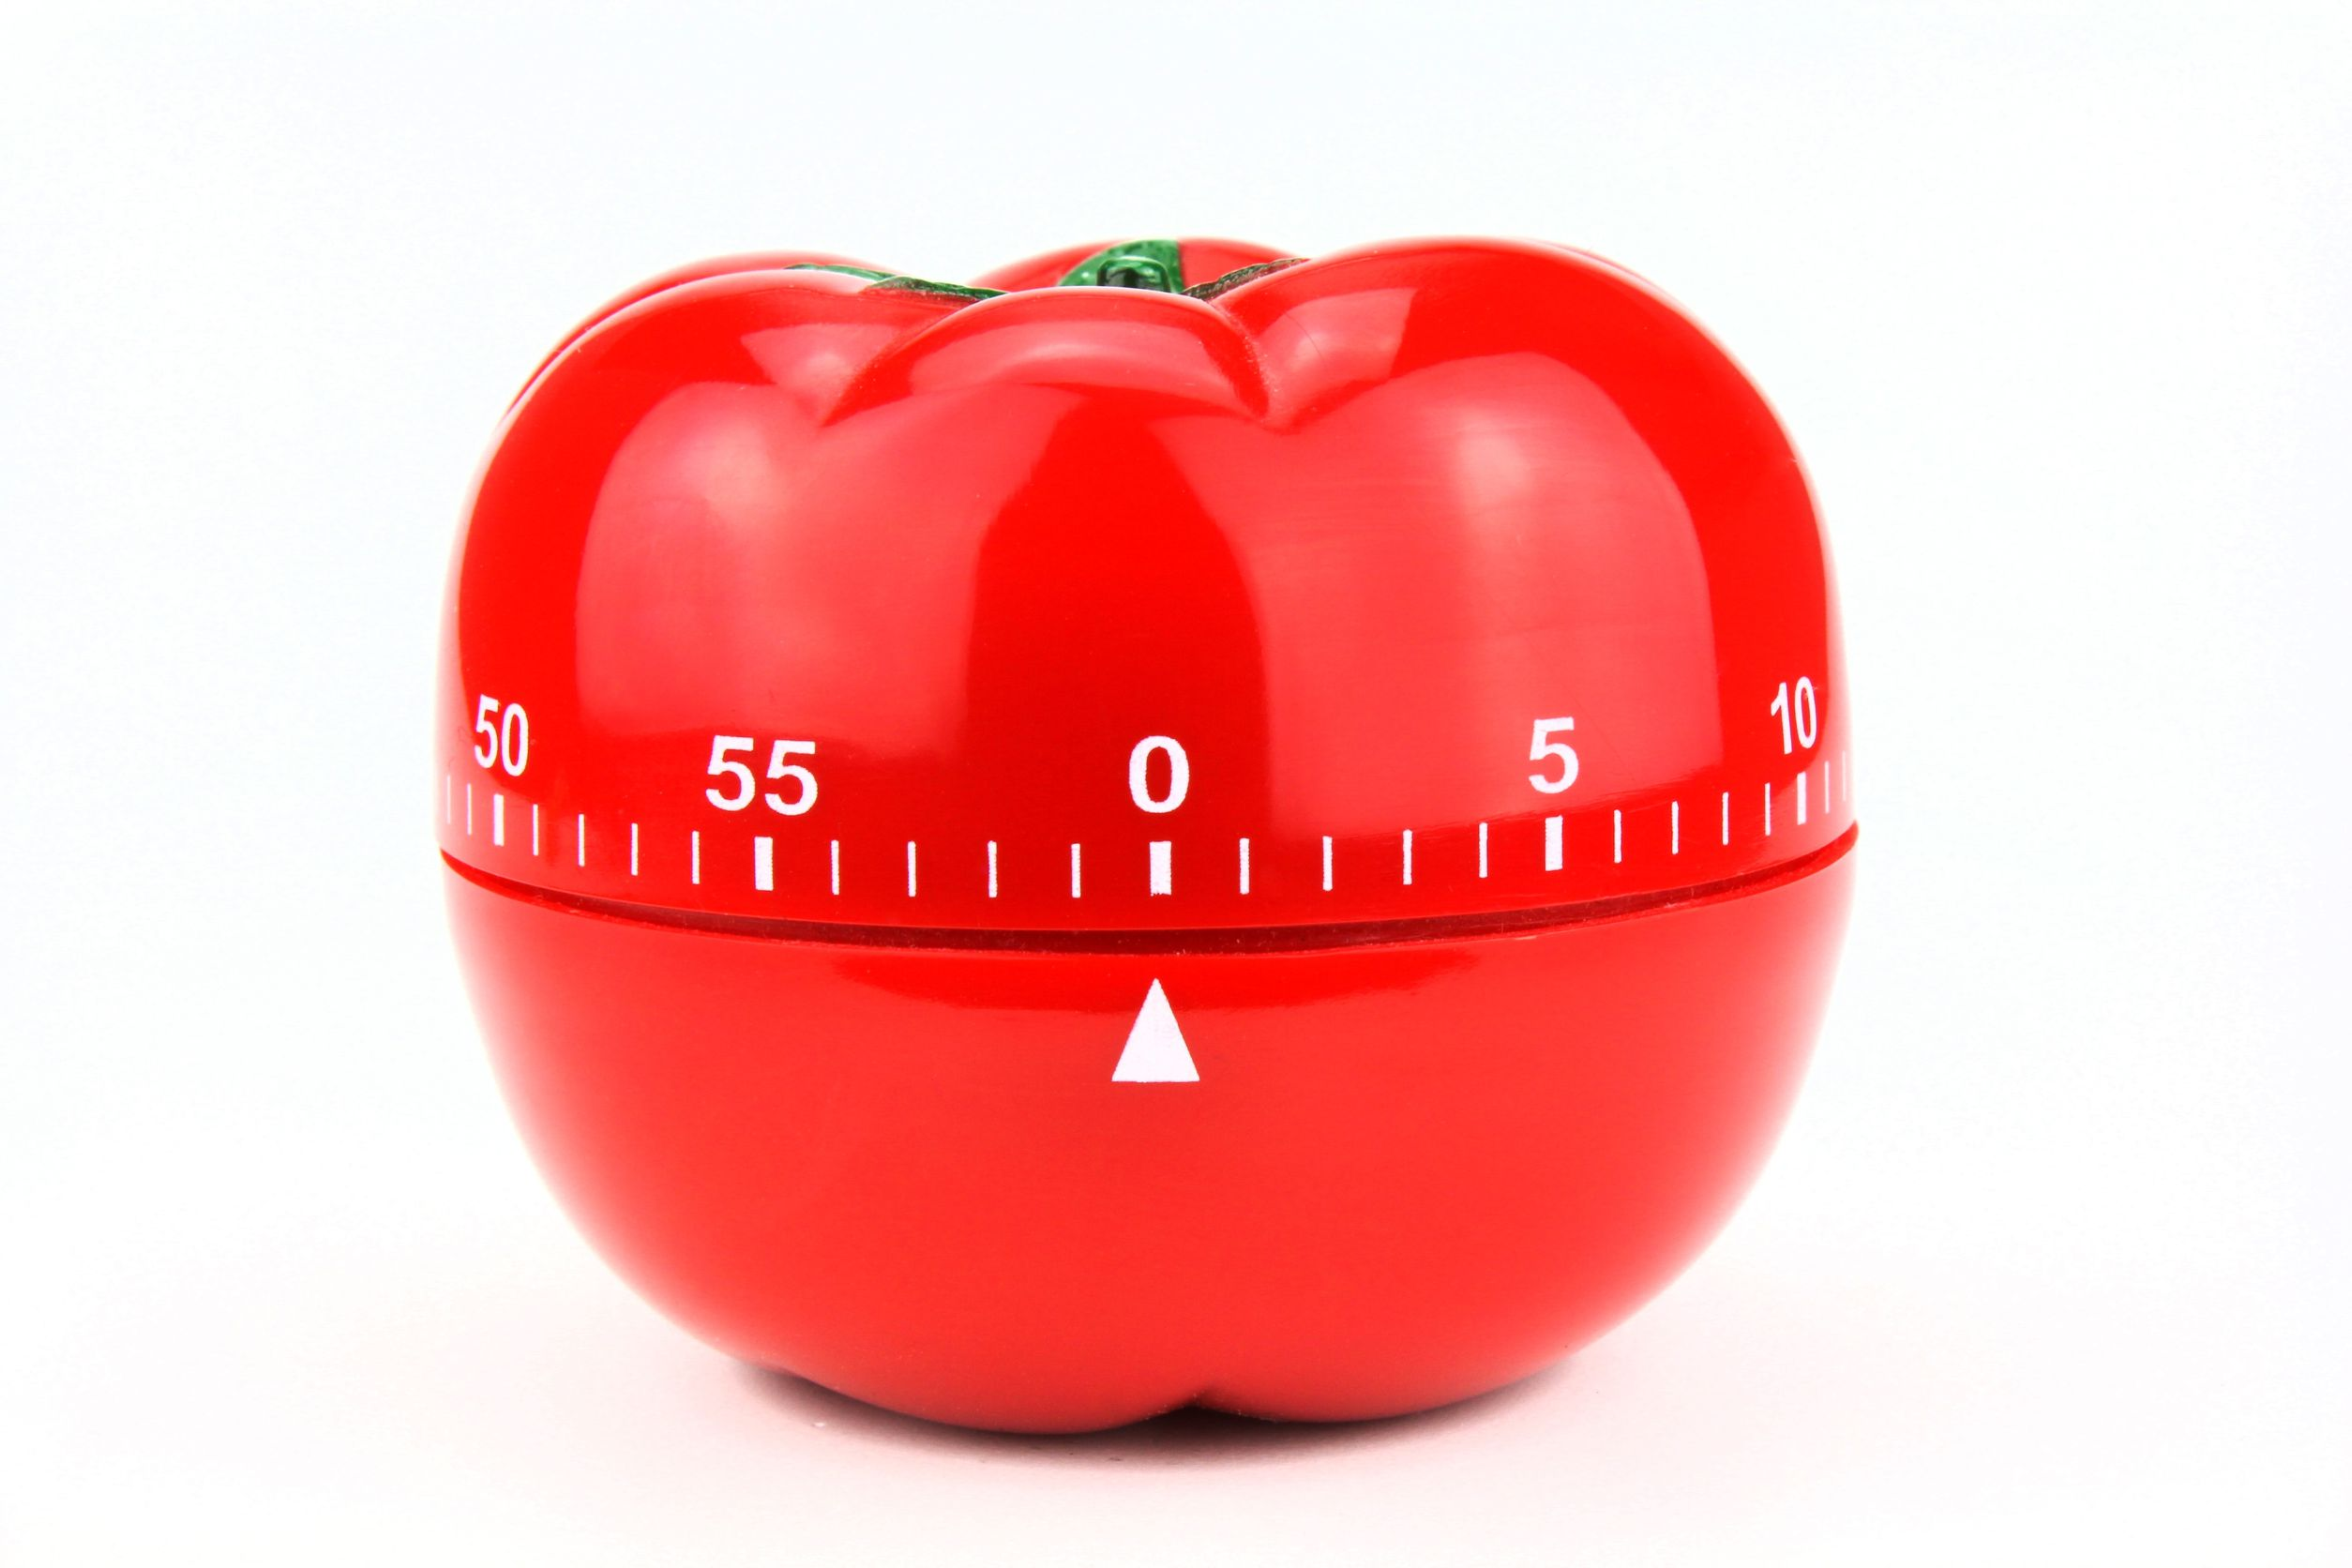
\includegraphics[width=0.40\textwidth]{./img/pomodoro.jpg} \hspace{0.2cm}
        
\includegraphics[width=0.40\textwidth]{./img/croissant.jpg} \\
        
\includegraphics[width=\textwidth]{../../report/src/img/mgs.png}
    \end{minipage}
\end{FrameWithSubSection}


\subsection{Gantt chart}
\begin{FrameWithSubSection}
    \hspace*{-0.8cm}
\begin{ganttchart}[
        x unit=0.35cm,
        y unit title=.4cm,
        y unit chart=.4cm,
        hgrid=true,
        vgrid={*1{red, dotted}},
        canvas/.style={fill=base2},
        bar/.style={fill=orange},
        title/.style={fill=base2},
        group/.style={fill=blue, shape=ganttgroup},
        bar height = 0.4,
        bar label font = {\scriptsize},
        title label font = {\color{blue}},
    ]{1}{24}
    \gantttitlelist[title label font={\tiny}]{1, ..., 24}{1} \\
    \ganttbar{Arrival, installation}{1}{1} \\
    \ganttgroup{\color{blue}Client deliverables}{4}{20} \\
    \ganttbar{Improving build process}{4}{11} \\
    \ganttbar{Multi-variant support}{5}{6} \\
    \ganttbar{Fixed point enhancements}{9}{11}\\
    \ganttbar{Multi modem support}{17}{20}\\
    \ganttgroup{\color{blue}Open-sourcing}{1}{20} \\
    \ganttbar{Newcomer documentation}{1}{4}\\
    \ganttbar{Intellectual property}{12}{13}\\
    \ganttbar{Alsa plugin refactor}{12}{14}\\
    \ganttbar{Filesystem plugin update}{14}{15}\\
    \ganttbar{Core update}{15}{18}\\
    \ganttbar{Alsa plugin update}{17}{20}\\
    \ganttgroup{\color{blue}University}{21}{24} \\
    \ganttbar{Internship report}{21}{24} \\
    \ganttbar{Slides internship}{23}{24}
\end{ganttchart}
\end{FrameWithSubSection}

